\begin{figure*}[tb!]
    \centering
    \subfloat[Energy, \( N = 1 \)]{
        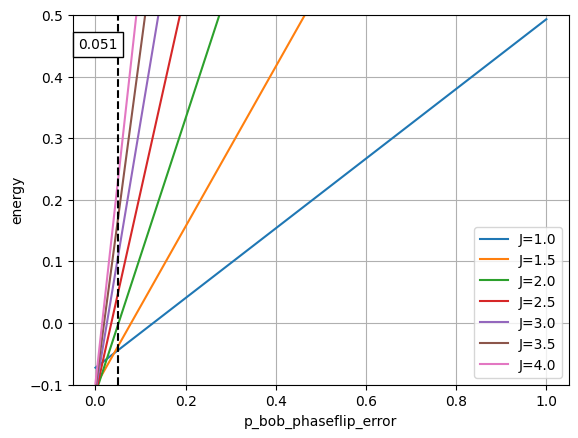
\includegraphics[width=0.225\textwidth]{Appendix/plots/errors/numerical/Alice/N1/N1_energy_vs_p_bob_phaseflip_error.png}
    }
    \hfill
    \subfloat[Energy, \( N = 2 \)]{
        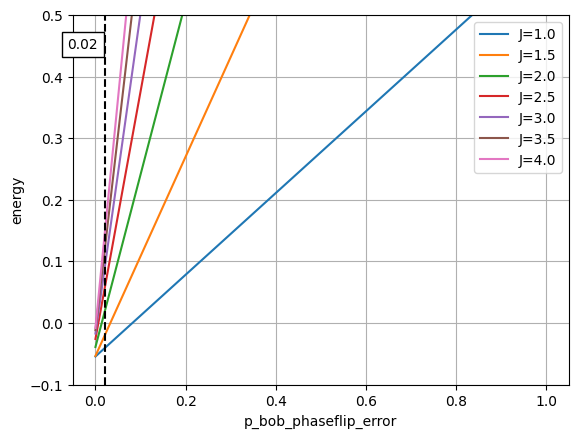
\includegraphics[width=0.225\textwidth]{Appendix/plots/errors/numerical/Alice/N2/N2_energy_vs_p_bob_phaseflip_error.png}
    }
    \hfill
    \subfloat[Energy, \( N = 3 \)]{
        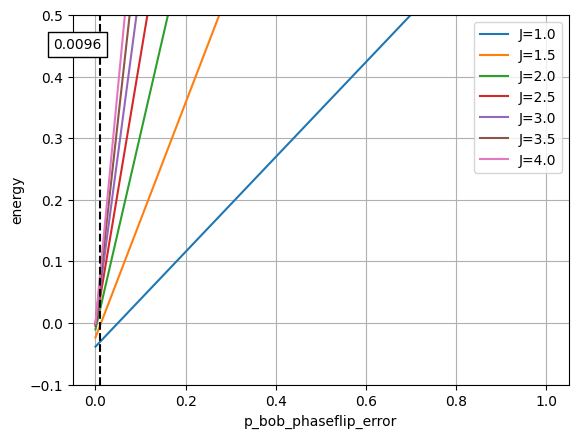
\includegraphics[width=0.225\textwidth]{Appendix/plots/errors/numerical/Alice/N3/N3_energy_vs_p_bob_phaseflip_error.png}
    }
    \hfill
    \subfloat[Energy, \( N = 4 \)]{
        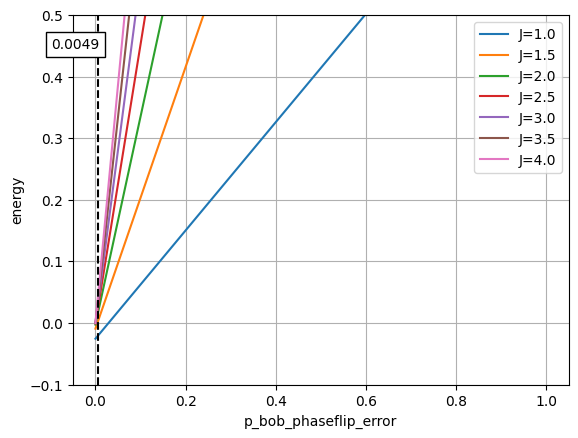
\includegraphics[width=0.225\textwidth]{Appendix/plots/errors/numerical/Alice/N4/N4_energy_vs_p_bob_phaseflip_error.png}
    }

    \vspace{0.5em}

    \subfloat[Charge, \( N = 1 \)]{
        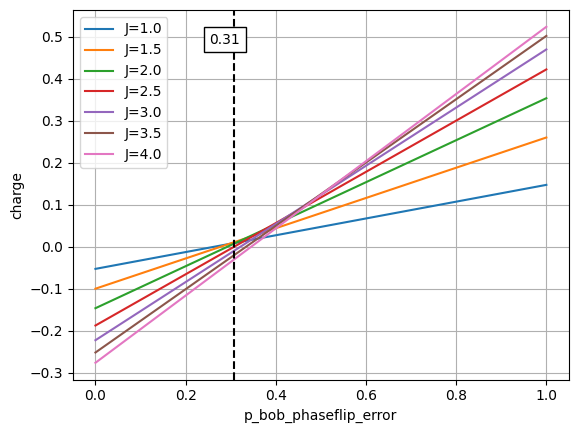
\includegraphics[width=0.225\textwidth]{Appendix/plots/errors/numerical/Alice/N1/N1_charge_vs_p_bob_phaseflip_error.png}
    }
    \hfill
    \subfloat[Charge, \( N = 2 \)]{
        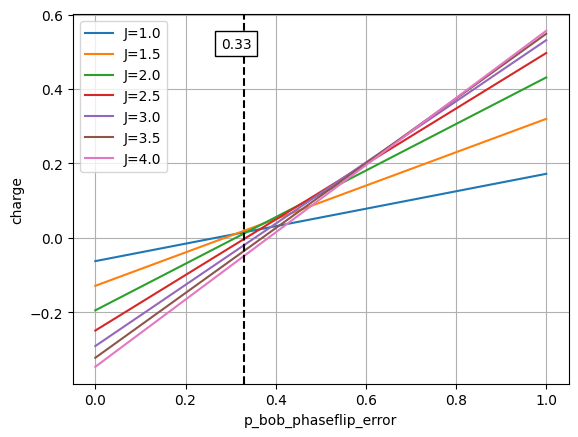
\includegraphics[width=0.225\textwidth]{Appendix/plots/errors/numerical/Alice/N2/N2_charge_vs_p_bob_phaseflip_error.png}
    }
    \hfill
    \subfloat[Charge, \( N = 3 \)]{
        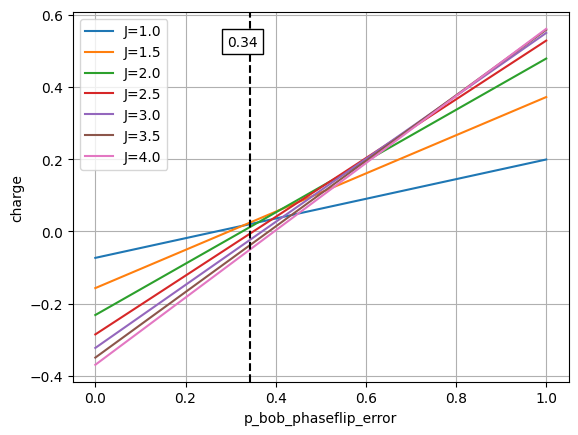
\includegraphics[width=0.225\textwidth]{Appendix/plots/errors/numerical/Alice/N3/N3_charge_vs_p_bob_phaseflip_error.png}
    }
    \hfill
    \subfloat[Charge, \( N = 4 \)]{
        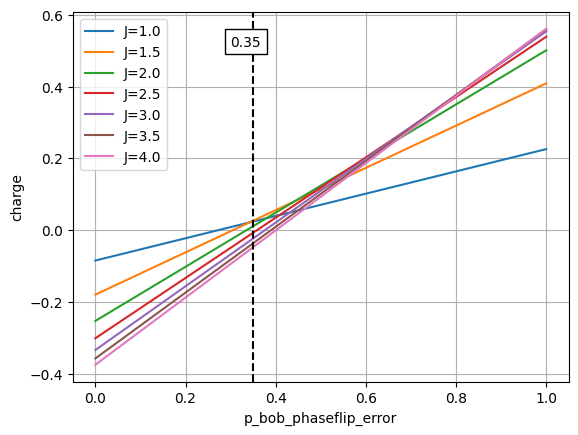
\includegraphics[width=0.225\textwidth]{Appendix/plots/errors/numerical/Alice/N4/N4_charge_vs_p_bob_phaseflip_error.png}
    }
    
    \caption{Numerical simulation results for teleported expectation value vs. the probability $p$ of phaseflip at Bob's site for Star-Interaction Hamiltonian \(H^{(1)}\).}
    \label{fig:alice_num_bob_phaseflip_error_appendix}
\end{figure*}

\begin{figure*}[tb!]
    \centering
    \subfloat[Energy, \( N = 1 \)]{
        
\includegraphics[width=0.3\textwidth]{Appendix/plots/errors/qiskit/Alice/N1/N1_energy_vs_p_bob_phaseflip_error.png}
    }
    \hfill
    \subfloat[Energy, \( N = 2 \)]{
        
\includegraphics[width=0.3\textwidth]{Appendix/plots/errors/qiskit/Alice/N2/N2_energy_vs_p_bob_phaseflip_error.png}
    }
    \hfill
    \subfloat[Energy, \( N = 3 \)]{
        
\includegraphics[width=0.3\textwidth]{Appendix/plots/errors/qiskit/Alice/N3/N3_energy_vs_p_bob_phaseflip_error.png}
    }

    \vspace{0.5em}

    \subfloat[Charge, \( N = 1 \)]{
        
\includegraphics[width=0.3\textwidth]{Appendix/plots/errors/qiskit/Alice/N1/N1_charge_vs_p_bob_phaseflip_error.png}
    }
    \hfill
    \subfloat[Charge, \( N = 2 \)]{
        
\includegraphics[width=0.3\textwidth]{Appendix/plots/errors/qiskit/Alice/N2/N2_charge_vs_p_bob_phaseflip_error.png}
    }
    \hfill
    \subfloat[Charge, \( N = 3 \)]{
        
\includegraphics[width=0.3\textwidth]{Appendix/plots/errors/qiskit/Alice/N3/N3_charge_vs_p_bob_phaseflip_error.png}
    }
    
    \caption{Qiskit simulation results for teleported expectation value vs. the probability $p$ of phaseflip at Bob's site for Star-Interaction Hamiltonian \(H^{(1)}\).}
    \label{fig:alice_qiskit_bob_phaseflip_error_appendix}
\end{figure*}

\begin{figure*}[tb!]
    \centering
    \subfloat[Energy, \( N = 2 \)]{
        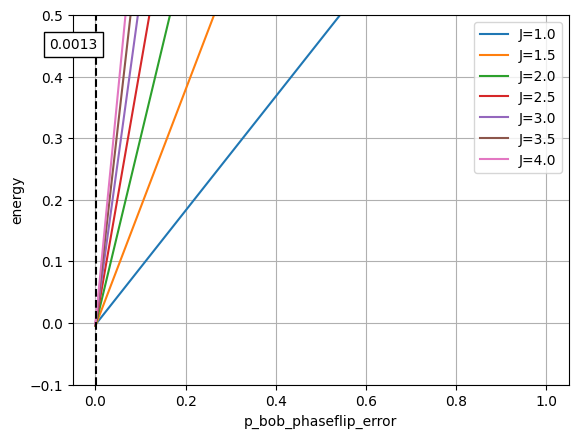
\includegraphics[width=0.3\textwidth]{Appendix/plots/errors/numerical/NearestNeighbors/N2/X_N2_energy_vs_p_bob_phaseflip_error.png}
    }
    \hfill
    \subfloat[Energy, \( N = 3 \)]{
        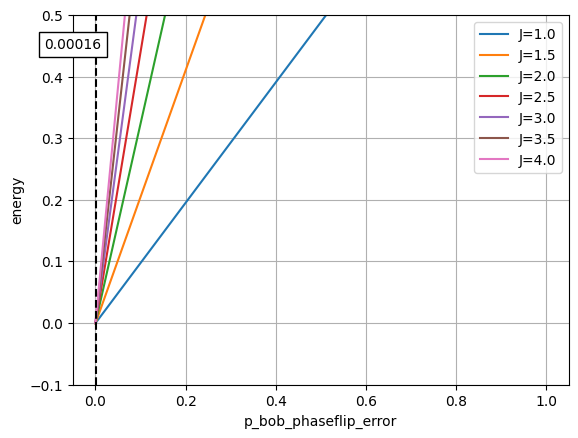
\includegraphics[width=0.3\textwidth]{Appendix/plots/errors/numerical/NearestNeighbors/N3/X_N3_energy_vs_p_bob_phaseflip_error.png}
    }
    \hfill
    \subfloat[Energy, \( N = 4 \)]{
        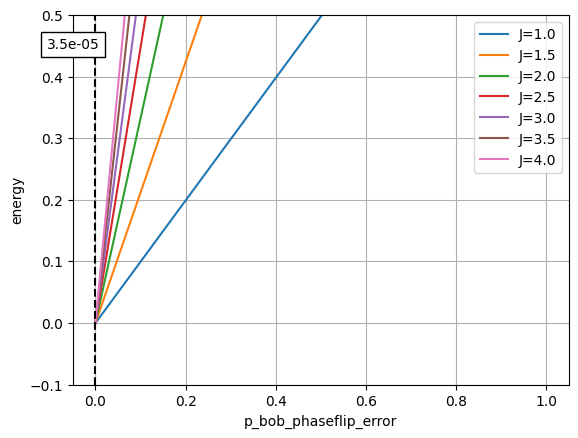
\includegraphics[width=0.3\textwidth]{Appendix/plots/errors/numerical/NearestNeighbors/N4/X_N4_energy_vs_p_bob_phaseflip_error.png}
    }

    \vspace{0.5em}

    \subfloat[Charge, \( N = 2 \)]{
        
\includegraphics[width=0.3\textwidth]{plots/errors/numerical/N2_charge_vs_p_bob_phaseflip_error.png}
    }
    \hfill
    \subfloat[Charge, \( N = 3 \)]{
        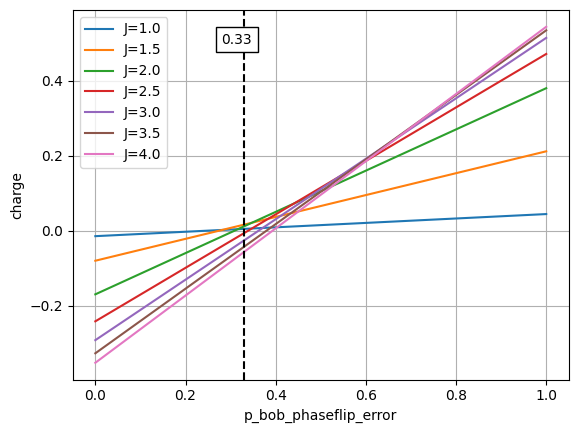
\includegraphics[width=0.3\textwidth]{Appendix/plots/errors/numerical/NearestNeighbors/N3/X_N3_charge_vs_p_bob_phaseflip_error.png}
    }
    \hfill
    \subfloat[Charge, \( N = 4 \)]{
        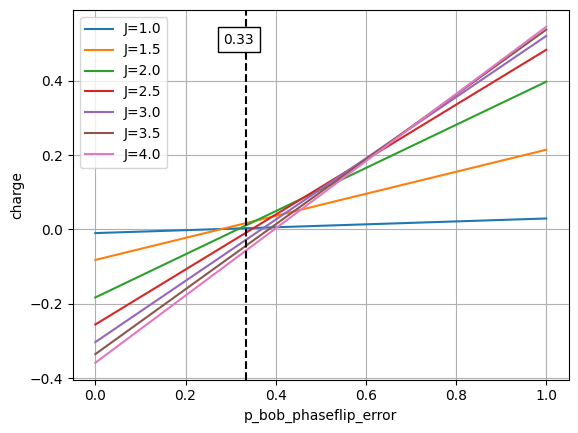
\includegraphics[width=0.3\textwidth]{Appendix/plots/errors/numerical/NearestNeighbors/N4/X_N4_charge_vs_p_bob_phaseflip_error.png}
    }
    
    \caption{Numerical simulation results for teleported expectation value vs. the probability $p$ of phaseflip at Bob's site for Nearest Neighbors Hamiltonian \(H^{(2)}\) with Alice base \(\sigma_A = X_0\).}
    \label{fig:nn_X_num_bob_phaseflip_error_appendix}
\end{figure*}

\begin{figure*}[tb!]
    \centering
    \subfloat[Energy, \( N = 2 \)]{
        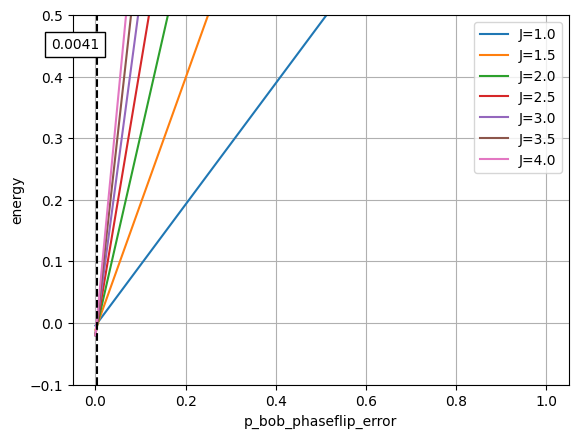
\includegraphics[width=0.3\textwidth]{Appendix/plots/errors/numerical/NearestNeighbors/N2/Y_N2_energy_vs_p_bob_phaseflip_error.png}
    }
    \hfill
    \subfloat[Energy, \( N = 3 \)]{
        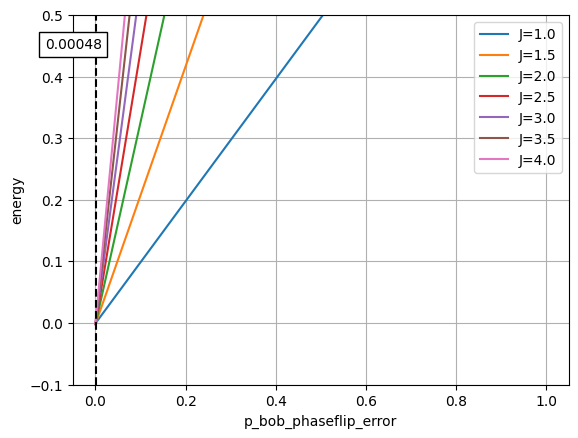
\includegraphics[width=0.3\textwidth]{Appendix/plots/errors/numerical/NearestNeighbors/N3/Y_N3_energy_vs_p_bob_phaseflip_error.png}
    }
    \hfill
    \subfloat[Energy, \( N = 4 \)]{
        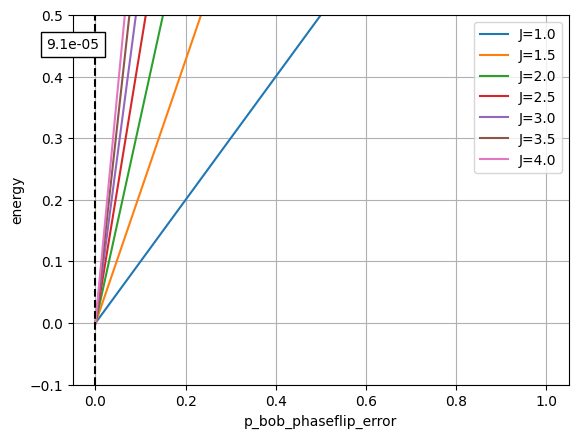
\includegraphics[width=0.3\textwidth]{Appendix/plots/errors/numerical/NearestNeighbors/N4/Y_N4_energy_vs_p_bob_phaseflip_error.png}
    }

    \vspace{0.5em}

    \subfloat[Charge, \( N = 2 \)]{
        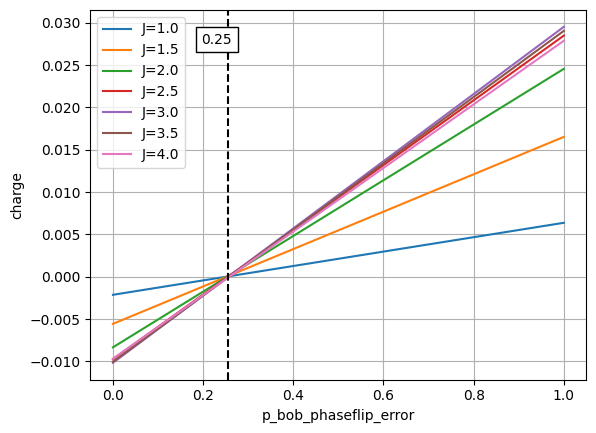
\includegraphics[width=0.3\textwidth]{Appendix/plots/errors/numerical/NearestNeighbors/N2/Y_N2_charge_vs_p_bob_phaseflip_error.png}
    }
    \hfill
    \subfloat[Charge, \( N = 3 \)]{
        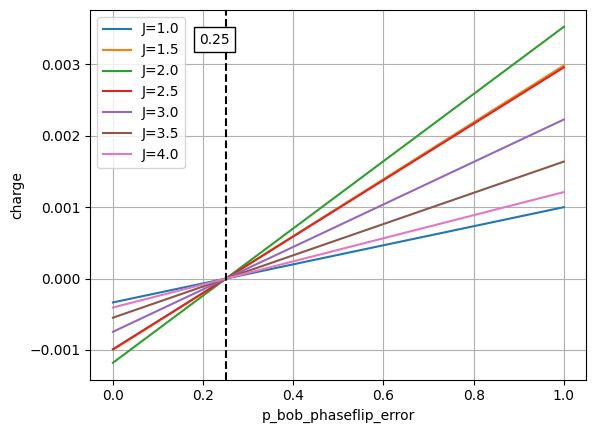
\includegraphics[width=0.3\textwidth]{Appendix/plots/errors/numerical/NearestNeighbors/N3/Y_N3_charge_vs_p_bob_phaseflip_error.png}
    }
    \hfill
    \subfloat[Charge, \( N = 4 \)]{
        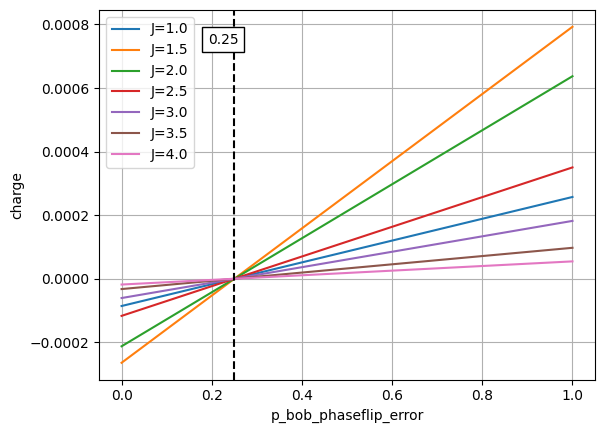
\includegraphics[width=0.3\textwidth]{Appendix/plots/errors/numerical/NearestNeighbors/N4/Y_N4_charge_vs_p_bob_phaseflip_error.png}
    }
    
    \caption{Numerical simulation results for teleported expectation value vs. the probability $p$ of phaseflip at Bob's site for Nearest Neighbors Hamiltonian \(H^{(2)}\) with Alice base \(\sigma_A = Y_0\).}
    \label{fig:nn_Y_num_bob_phaseflip_error_appendix}
\end{figure*}

\begin{figure*}[tb!]
    \centering
    \subfloat[Energy, \( N = 2 \), \( \sigma_A = X_0 \)]{
        
\includegraphics[width=0.225\textwidth]{Appendix/plots/errors/qiskit/NearestNeighbors/N2/X_N2_energy_vs_p_bob_phaseflip_error.png}
    }
    \hfill
    \subfloat[Energy, \( N = 3 \), \( \sigma_A = X_0 \)]{
        
\includegraphics[width=0.225\textwidth]{Appendix/plots/errors/qiskit/NearestNeighbors/N3/X_N3_energy_vs_p_bob_phaseflip_error.png}
    }
    \hfill
    \subfloat[Charge, \( N = 2 \), \( \sigma_A = X_0 \)]{
        
\includegraphics[width=0.225\textwidth]{plots/errors/qiskit/N2_charge_vs_p_bob_phaseflip_error.png}
    }
    \hfill
    \subfloat[Charge, \( N = 3 \), \( \sigma_A = X_0 \)]{
        
\includegraphics[width=0.225\textwidth]{Appendix/plots/errors/qiskit/NearestNeighbors/N3/X_N3_charge_vs_p_bob_phaseflip_error.png}
    }

    \vspace{0.5em}

    \subfloat[Energy, \( N = 2 \), \( \sigma_A = Y_0 \)]{
        
\includegraphics[width=0.225\textwidth]{Appendix/plots/errors/qiskit/NearestNeighbors/N2/Y_N2_energy_vs_p_bob_phaseflip_error.png}
    }
    \hfill
    \subfloat[Energy, \( N = 3 \), \( \sigma_A = Y_0 \)]{
        
\includegraphics[width=0.225\textwidth]{Appendix/plots/errors/qiskit/NearestNeighbors/N3/Y_N3_energy_vs_p_bob_phaseflip_error.png}
    }
    \hfill
    \subfloat[Charge, \( N = 2 \), \( \sigma_A = Y_0 \)]{
        
\includegraphics[width=0.225\textwidth]{Appendix/plots/errors/qiskit/NearestNeighbors/N2/Y_N2_charge_vs_p_bob_phaseflip_error.png}
    }
    \hfill
    \subfloat[Charge, \( N = 3 \), \( \sigma_A = Y_0 \)]{
        
\includegraphics[width=0.225\textwidth]{Appendix/plots/errors/qiskit/NearestNeighbors/N3/Y_N3_charge_vs_p_bob_phaseflip_error.png}
    }
    
    \caption{Qiskit simulation results for teleported expectation value vs. the probability $p$ of phaseflip at Bob's site for Nearest Neighbors Hamiltonian \(H^{(2)}\) for both Alice bases.}
    \label{fig:nn_qiskit_bob_phaseflip_error_appendix}
\end{figure*}
